\chapter{AX.25}

AX.25 is the amateur radio derivative of CCITT X.25 that was designed during the early 1980's 
as the primary data link protocol used by amateur packet networks.
The AX.25 specification has been maintained by the Tucson Amateur Packet Radio (TAPR) 
organization until its latest release, Version 2.2 in July of 1998. 

The most significant difference between AX.25 and the original X.25 protocol lies
in the hardware addresses used by AX.25, which are based on the expectation of
each station using their FCC issues callsign. 
Each node is addressed by their callsign plus an additional 4 bit 
secondary station identifier (SSID), which allows each licensee to maintain and operate 
up to 16 stations in each packet namespace.

AX.25 is one of the best-documented protocols used in amateur radio packet networks,
so it could be argued that a chapter in this thesis considering AX.25 could be omitted.
The AX.25 specification goes into tremendous detail as to the expected behavior of each
node and how the system should transition between states.
Where documentation does fall short is in how APRS abuses a small subset of 
the AX.25 protocol for the specific needs of the APRS network.
The rest of the chapter will walk through each field of the AX.25 packet and
note how it is used by APRS, followed by a discussion of the implications of the FCC
requirement to identify an active transmitter by its FCC-issued license every ten minutes.

\section{Header Format for APRS}

A very limited subset of the complete AX.25 protocol is used by APRS due to APRS 
deliberately avoiding the use of any of the connected or control modes of AX.25. This 
means that any AX.25 protocol stack used for APRS need only support Unnumbered Information (UI)
frames, and many APRS protocol stacks cannot handle any other forms of AX.25 traffic. 
Figure \ref{fig:ax25uiformat} presents the modified form of the AX.25 frame that is used
by APRS.

\begin{figure}
	\centering
	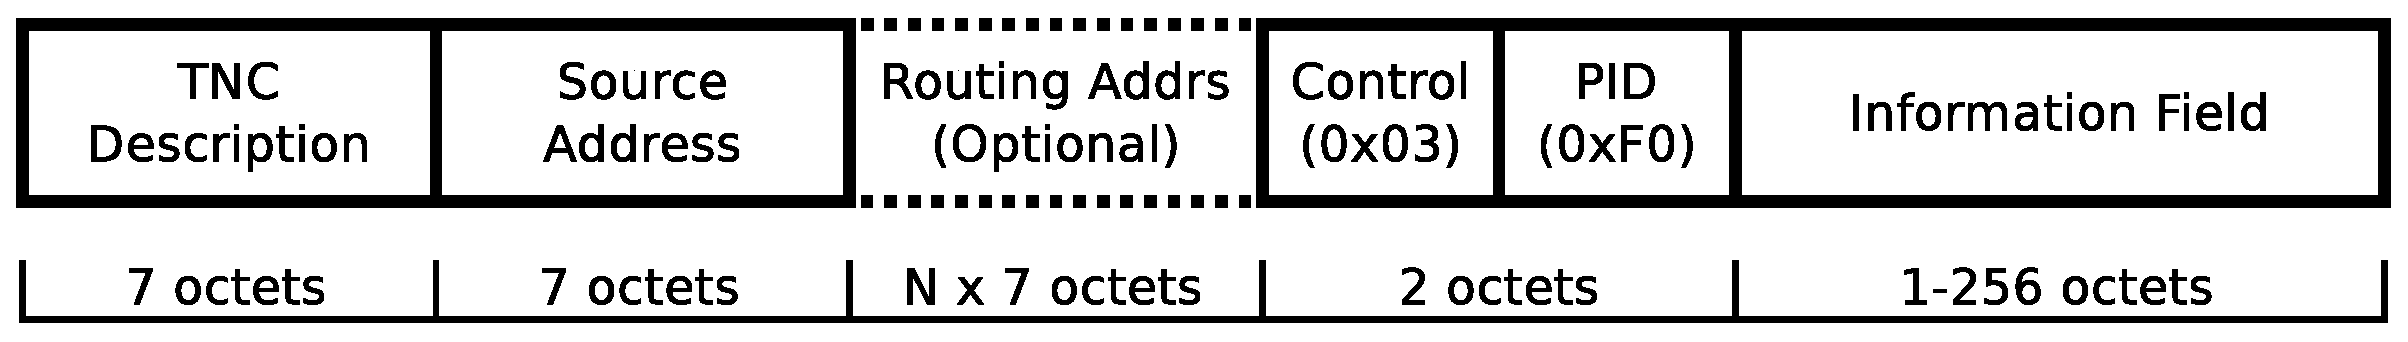
\includegraphics[width=1.0\textwidth]{src/dia/ax25ui}
	\caption{AX.25 UI Packet Format}
	\label{fig:ax25uiformat}
\end{figure}

\subsection{TNC Description / Destination Address}

Traditional AX.25 traffic is usually directed at a single station, which would be indicated by 
a packet's destination address. 
Since APRS is strictly a one-to-many network protocol at Layer 3, this field
was deemed not needed for APRS and several alternative uses for the field have been proposed.

The most popular application for this field is to be used as a tracker identifier, where a
six character identifier is allocated from the APRS Working Group to identify a specific 
APRS TNC and firmware version. 
This provides valuable information to the rest of the APRS network.
APRS
TNCs often ``misbehave" and it is helpful to be able to immediately identify the original
developer for a remote APRS node. 
Experimental trackers which have not yet received a tracker ID may use the 
APZ prefix with three additional arbitrary alphanumeric characters as their TNC identifier.

\subsection{Source Address}

The source address is either the FCC-issued or a ``tactical" callsign used by 
the beaconing APRS station, with an 
additional SSID appended to the station, which may range from zero to 15. Source addresses must 
be at least three characters long, and may not be any longer than six. Stations using AX.25 
over RF are limited to the SSID's of 0 to 15 due to AX.25's binary format, 
while APRS imposes a looser standard such that the SSID is only limited to 
two alphanumeric characters when not transported over AX.25 links..

\subsection{Routing Path}
\label{subsec:ax25RoutingPath}

The AX.25 routing path is an optional variable-length field consisting of an ordered list of
digipeaters which should process and re-transmit the considered packet. Should a station not
require the use of this field, it can be completely omitted and the end-of-path bit should be
set on the source address field. The path must consist of an integer number of seven octets.

The original AX.25 version 2.0 spec allowed for anywhere from zero to eight digipeaters to
be included in an AX.25 frame. Unfortunately, due to the unreliable nature of amateur 
packet radio, packets with a routing path requesting as many as eight hops would rarely be 
successfully delivered to the end station.
The version 2.2 specification for AX.25 was
rewritten limiting the number of requested digipeaters to two with the argument that packets
traveling beyond two hops should be handled by a higher layer protocol than AX.25.
Because AX.25 doesn't guarantee delivery from a digipeater to another station,
packets passing through a digipeater that are lost need to be
resent from their origin.
Higher layer protocols can recover from a lost packet locally 
without needing to twice consume
the bandwidth used to get the packet to the digipeater.

This concept of higher-layer retries and a limit of two digipeaters
introduced in AX.25 v2.2 is ignored by APRS.
More than two digipeaters are often seen on APRS traffic, 
and users are only strongly discouraged from using a large number of hops.

\subsection{Control Flags}

The Control Flag octet indicates different modes for the AX.25 frame.
Since APRS strictly uses only Unnumbered Information (UI) frames, this field must
contain the value 0x03.

\subsection{Protocol IDentifier}

The Protocol IDentifier (PID) field is normally used to identify the Layer 3 protocol
being transported by AX.25. TAPR has reportedly stopped processing requests for new PID
values to be issued to new Layer 3 applications of AX.25 \cite{millernopid}, 
which is a possible explanation for why APRS doesn't have a unique PID.
It instead uses the value of 0xF0, incorrectly indicating that no Layer 3 protocol is in use.

\subsection{Information Field}

The rest of the AX.25 frame contains the APRS payload in
what is called the Information Field.
The end of the Information Field is indicated by the Layer 1 modulation, which is traditionally
the Amateur Bell 202 FCS and 0x7E flag.

The maximum transmission unit for the Information Field is 256 octets, and APRS imposes
a minimum of one octet identifying the type of APRS packet being carried \cite{aprsspec}.

\section{FCC Identification Requirements}

One of the conditions of operating a radio under FCC Title 47 CFR Part 97 is that amateur radio 
operators are required to transmit their callsign at least once every ten minutes while active.
An ongoing source of controversy in the APRS community is what this means for operating
an APRS node, and particularly digipeaters.

The source of argument is what constitutes properly identifying the
transmitting station; only a station's FCC callsign in the source address field,
or simply including the callsign somewhere in the complete frame.
Considering only the source address field as a valid way to identify a station is
a very conservative interpretation of \S97.119, but establishes the requirement that every 
digipeater active in the APRS network needs to originate a new packet every ten minutes.
Alternatively, accepting the digipeater's callsign injected anywhere in an outgoing 
packet lends itself to the digipeater staying more ``quiet" since appending its callsign
to the end of the routing path of incoming packets could be considered identification enough.

The considered disadvantage of the more conservative interpretation is that the additional
beacons being generated by every active digipeater every ten minutes is an
excessive burden on the APRS network. Digipeaters rarely have information of value
to the rest of the APRS network, so their beacons are seen as little more than noise.
This interpretation also prohibits the use of ``tactical" callsigns, which are selected
to convey more useful information that the control operator's callsign.
One common example is digipeaters on major mountain peaks; a digipeater 
on Tassajara peak beaconing as ``TASS" has a more meaningful name than beaconing as
its owner's FCC callsign. The FCC callsign is then placed somewhere in the comment section
of the APRS beacon.

The issue with identifying via appending callsigns to other station's packets and
using tactical callsigns is that it isn't always clear what a station's callsign is.
\begin{itemize}
	\item Many digipeaters fail to correctly append their callsign to routing paths when
		they process packets, so the last callsign in the path isn't necessarily the 
		station transmitting it.
	\item There is no standard secondary place for a station's ``real" callsign 
		when using a tactical call.
		Operators often program digipeaters with comments that fail to make it clear
		what their callsign actually is.
\end{itemize}

In the end, the question of how each station needs to identify to meet part 97 is a
strictly legal one. Arguments have been made for interpreting \S97.119 
several places between these two extremes, and the final decision on how to interpret
the legal requirements are left up to the individual amateur radio operators and the
federal government's lawyers.

